% Created by tikzDevice version 0.12.3 on 2020-10-09 09:34:57
% !TEX encoding = UTF-8 Unicode
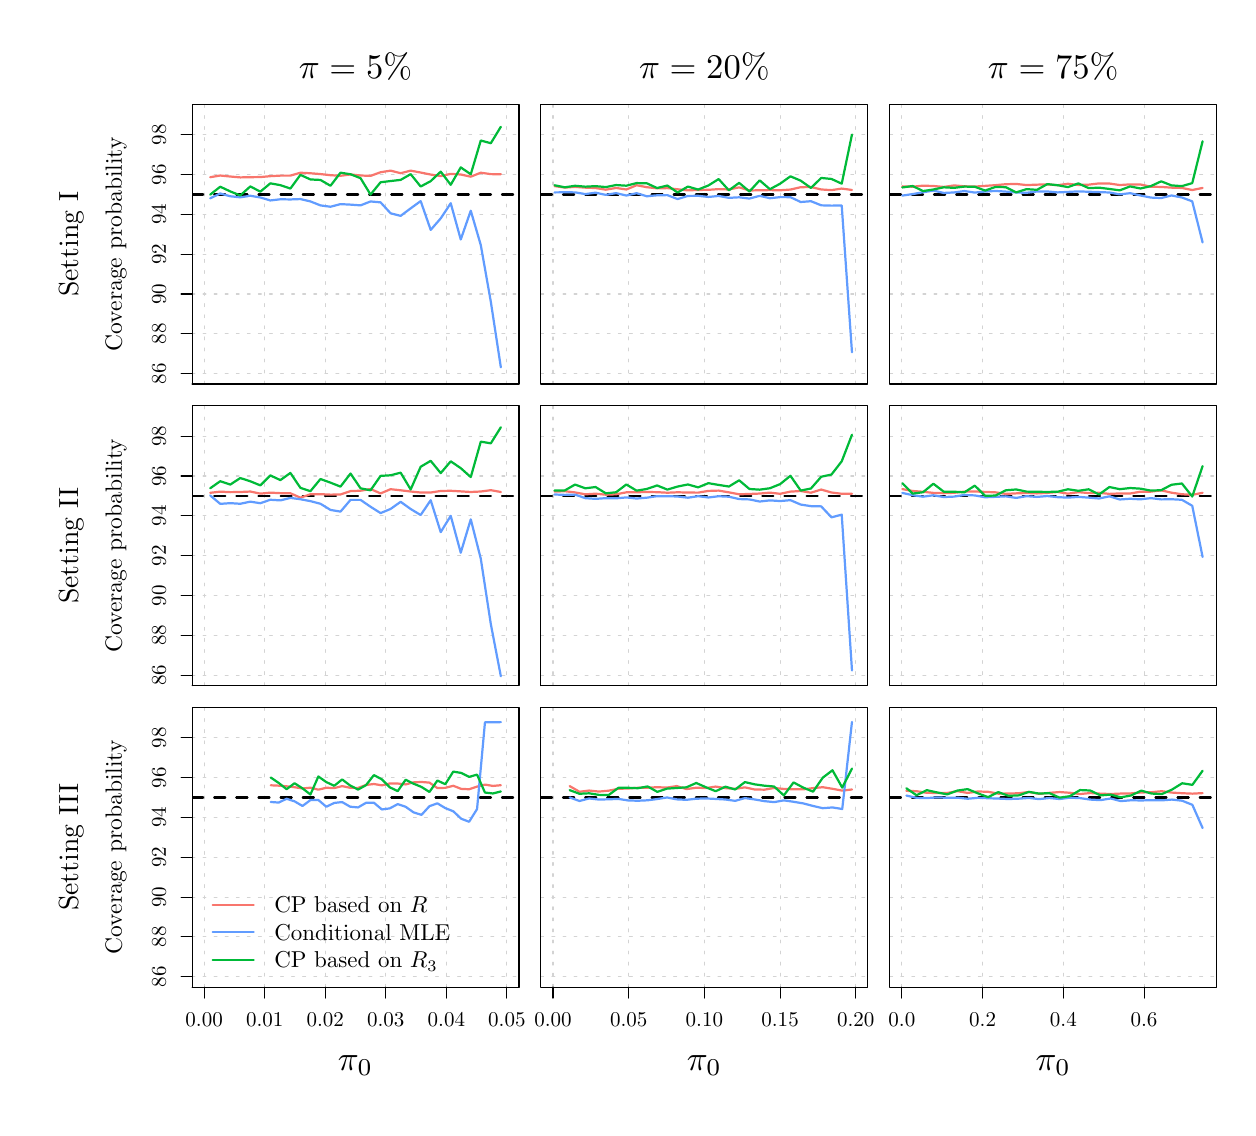
\begin{tikzpicture}[x=1pt,y=1pt]
\definecolor{fillColor}{RGB}{255,255,255}
\path[use as bounding box,fill=fillColor,fill opacity=0.00] (0,0) rectangle (433.62,390.26);
\begin{scope}
\path[clip] ( 55.44,257.53) rectangle (181.50,366.50);
\definecolor{drawColor}{RGB}{0,0,0}

\node[text=drawColor,anchor=base,inner sep=0pt, outer sep=0pt, scale=  0.66] at (118.47,231.40) {Simulation ID};

\node[text=drawColor,rotate= 90.00,anchor=base,inner sep=0pt, outer sep=0pt, scale=  0.66] at ( 34.06,312.01) {Ratio of RMSE};
\end{scope}
\begin{scope}
\path[clip] (  0.00,  0.00) rectangle (433.62,390.26);
\definecolor{drawColor}{RGB}{0,0,0}

\path[draw=drawColor,line width= 0.4pt,line join=round,line cap=round] ( 59.40,265.23) -- ( 59.40,351.60);

\path[draw=drawColor,line width= 0.4pt,line join=round,line cap=round] ( 59.40,265.23) -- ( 55.44,265.23);

\path[draw=drawColor,line width= 0.4pt,line join=round,line cap=round] ( 59.40,279.63) -- ( 55.44,279.63);

\path[draw=drawColor,line width= 0.4pt,line join=round,line cap=round] ( 59.40,294.02) -- ( 55.44,294.02);

\path[draw=drawColor,line width= 0.4pt,line join=round,line cap=round] ( 59.40,308.42) -- ( 55.44,308.42);

\path[draw=drawColor,line width= 0.4pt,line join=round,line cap=round] ( 59.40,322.81) -- ( 55.44,322.81);

\path[draw=drawColor,line width= 0.4pt,line join=round,line cap=round] ( 59.40,337.20) -- ( 55.44,337.20);

\path[draw=drawColor,line width= 0.4pt,line join=round,line cap=round] ( 59.40,351.60) -- ( 55.44,351.60);

\node[text=drawColor,rotate= 90.00,anchor=base,inner sep=0pt, outer sep=0pt, scale=  0.76] at ( 49.90,265.23) {86};

\node[text=drawColor,rotate= 90.00,anchor=base,inner sep=0pt, outer sep=0pt, scale=  0.76] at ( 49.90,279.63) {88};

\node[text=drawColor,rotate= 90.00,anchor=base,inner sep=0pt, outer sep=0pt, scale=  0.76] at ( 49.90,294.02) {90};

\node[text=drawColor,rotate= 90.00,anchor=base,inner sep=0pt, outer sep=0pt, scale=  0.76] at ( 49.90,308.42) {92};

\node[text=drawColor,rotate= 90.00,anchor=base,inner sep=0pt, outer sep=0pt, scale=  0.76] at ( 49.90,322.81) {94};

\node[text=drawColor,rotate= 90.00,anchor=base,inner sep=0pt, outer sep=0pt, scale=  0.76] at ( 49.90,337.20) {96};

\node[text=drawColor,rotate= 90.00,anchor=base,inner sep=0pt, outer sep=0pt, scale=  0.76] at ( 49.90,351.60) {98};
\end{scope}
\begin{scope}
\path[clip] ( 59.40,261.49) rectangle (177.54,362.54);
\definecolor{drawColor}{RGB}{211,211,211}

\path[draw=drawColor,line width= 0.4pt,dash pattern=on 1pt off 3pt ,line join=round,line cap=round] ( 63.78,261.49) -- ( 63.78,362.54);

\path[draw=drawColor,line width= 0.4pt,dash pattern=on 1pt off 3pt ,line join=round,line cap=round] ( 85.65,261.49) -- ( 85.65,362.54);

\path[draw=drawColor,line width= 0.4pt,dash pattern=on 1pt off 3pt ,line join=round,line cap=round] (107.53,261.49) -- (107.53,362.54);

\path[draw=drawColor,line width= 0.4pt,dash pattern=on 1pt off 3pt ,line join=round,line cap=round] (129.41,261.49) -- (129.41,362.54);

\path[draw=drawColor,line width= 0.4pt,dash pattern=on 1pt off 3pt ,line join=round,line cap=round] (151.29,261.49) -- (151.29,362.54);

\path[draw=drawColor,line width= 0.4pt,dash pattern=on 1pt off 3pt ,line join=round,line cap=round] (173.16,261.49) -- (173.16,362.54);

\path[draw=drawColor,line width= 0.4pt,dash pattern=on 1pt off 3pt ,line join=round,line cap=round] ( 59.40,265.23) -- (177.54,265.23);

\path[draw=drawColor,line width= 0.4pt,dash pattern=on 1pt off 3pt ,line join=round,line cap=round] ( 59.40,279.63) -- (177.54,279.63);

\path[draw=drawColor,line width= 0.4pt,dash pattern=on 1pt off 3pt ,line join=round,line cap=round] ( 59.40,294.02) -- (177.54,294.02);

\path[draw=drawColor,line width= 0.4pt,dash pattern=on 1pt off 3pt ,line join=round,line cap=round] ( 59.40,308.42) -- (177.54,308.42);

\path[draw=drawColor,line width= 0.4pt,dash pattern=on 1pt off 3pt ,line join=round,line cap=round] ( 59.40,322.81) -- (177.54,322.81);

\path[draw=drawColor,line width= 0.4pt,dash pattern=on 1pt off 3pt ,line join=round,line cap=round] ( 59.40,337.20) -- (177.54,337.20);

\path[draw=drawColor,line width= 0.4pt,dash pattern=on 1pt off 3pt ,line join=round,line cap=round] ( 59.40,351.60) -- (177.54,351.60);
\end{scope}
\begin{scope}
\path[clip] (  0.00,  0.00) rectangle (433.62,390.26);
\definecolor{drawColor}{RGB}{0,0,0}

\path[draw=drawColor,line width= 0.4pt,line join=round,line cap=round] ( 59.40,261.49) --
	(177.54,261.49) --
	(177.54,362.54) --
	( 59.40,362.54) --
	( 59.40,261.49);
\end{scope}
\begin{scope}
\path[clip] ( 59.40,261.49) rectangle (177.54,362.54);
\definecolor{drawColor}{RGB}{0,0,0}

\path[draw=drawColor,line width= 0.8pt,dash pattern=on 4pt off 4pt ,line join=round,line cap=round] ( 59.40,330.01) -- (177.54,330.01);
\definecolor{drawColor}{RGB}{248,118,109}

\path[draw=drawColor,line width= 0.8pt,line join=round,line cap=round] ( 65.96,336.23) --
	( 69.58,336.83) --
	( 73.21,336.47) --
	( 76.83,336.15) --
	( 80.45,336.23) --
	( 84.07,336.27) --
	( 87.69,336.60) --
	( 91.31,336.79) --
	( 94.93,336.80) --
	( 98.55,337.84) --
	(102.17,337.65) --
	(105.80,337.35) --
	(109.42,336.95) --
	(113.04,336.73) --
	(116.66,337.22) --
	(120.28,336.84) --
	(123.90,336.70) --
	(127.52,338.02) --
	(131.14,338.59) --
	(134.77,337.67) --
	(138.39,338.59) --
	(142.01,337.91) --
	(145.63,337.18) --
	(149.25,336.64) --
	(152.87,337.43) --
	(156.49,337.20) --
	(160.11,336.41) --
	(163.73,337.85) --
	(167.36,337.33) --
	(170.98,337.32);
\definecolor{drawColor}{RGB}{97,156,255}

\path[draw=drawColor,line width= 0.8pt,line join=round,line cap=round] ( 65.96,328.58) --
	( 69.58,330.35) --
	( 73.21,329.33) --
	( 76.83,328.96) --
	( 80.45,329.52) --
	( 84.07,328.90) --
	( 87.69,327.82) --
	( 91.31,328.25) --
	( 94.93,328.19) --
	( 98.55,328.32) --
	(102.17,327.47) --
	(105.80,326.03) --
	(109.42,325.55) --
	(113.04,326.50) --
	(116.66,326.31) --
	(120.28,326.05) --
	(123.90,327.46) --
	(127.52,327.13) --
	(131.14,323.18) --
	(134.77,322.25) --
	(138.39,324.96) --
	(142.01,327.59) --
	(145.63,317.18) --
	(149.25,321.34) --
	(152.87,326.81) --
	(156.49,313.71) --
	(160.11,324.11) --
	(163.73,311.70) --
	(167.36,291.20) --
	(170.98,267.52);
\definecolor{drawColor}{RGB}{0,186,56}

\path[draw=drawColor,line width= 0.8pt,line join=round,line cap=round] ( 65.96,329.91) --
	( 69.58,332.79) --
	( 73.21,331.09) --
	( 76.83,329.62) --
	( 80.45,332.90) --
	( 84.07,331.00) --
	( 87.69,334.01) --
	( 91.31,333.35) --
	( 94.93,332.12) --
	( 98.55,337.06) --
	(102.17,335.41) --
	(105.80,335.23) --
	(109.42,333.12) --
	(113.04,337.85) --
	(116.66,337.29) --
	(120.28,335.87) --
	(123.90,329.95) --
	(127.52,334.40) --
	(131.14,334.84) --
	(134.77,335.25) --
	(138.39,337.33) --
	(142.01,332.86) --
	(145.63,334.80) --
	(149.25,338.23) --
	(152.87,333.48) --
	(156.49,339.77) --
	(160.11,337.29) --
	(163.73,349.48) --
	(167.36,348.50) --
	(170.98,354.46);
\end{scope}
\begin{scope}
\path[clip] (  0.00,  0.00) rectangle (433.62,390.26);
\definecolor{drawColor}{RGB}{0,0,0}

\node[text=drawColor,rotate= 90.00,anchor=base,inner sep=0pt, outer sep=0pt, scale=  1.00] at ( 18.22,312.01) {Setting I};

\node[text=drawColor,rotate= 90.00,anchor=base,inner sep=0pt, outer sep=0pt, scale=  0.85] at ( 34.06,312.01) {Coverage probability};

\node[text=drawColor,anchor=base,inner sep=0pt, outer sep=0pt, scale=  1.25] at (118.47,372.04) {$\pi = 5\%$};
\end{scope}
\begin{scope}
\path[clip] (181.50,257.53) rectangle (307.56,366.50);
\definecolor{drawColor}{RGB}{0,0,0}

\node[text=drawColor,anchor=base,inner sep=0pt, outer sep=0pt, scale=  0.66] at (244.53,231.40) {Simulation ID};

\node[text=drawColor,rotate= 90.00,anchor=base,inner sep=0pt, outer sep=0pt, scale=  0.66] at (160.12,312.01) {Ratio of RMSE};
\end{scope}
\begin{scope}
\path[clip] (185.46,261.49) rectangle (303.60,362.54);
\definecolor{drawColor}{RGB}{211,211,211}

\path[draw=drawColor,line width= 0.4pt,dash pattern=on 1pt off 3pt ,line join=round,line cap=round] (189.84,261.49) -- (189.84,362.54);

\path[draw=drawColor,line width= 0.4pt,dash pattern=on 1pt off 3pt ,line join=round,line cap=round] (217.18,261.49) -- (217.18,362.54);

\path[draw=drawColor,line width= 0.4pt,dash pattern=on 1pt off 3pt ,line join=round,line cap=round] (244.53,261.49) -- (244.53,362.54);

\path[draw=drawColor,line width= 0.4pt,dash pattern=on 1pt off 3pt ,line join=round,line cap=round] (271.88,261.49) -- (271.88,362.54);

\path[draw=drawColor,line width= 0.4pt,dash pattern=on 1pt off 3pt ,line join=round,line cap=round] (299.22,261.49) -- (299.22,362.54);

\path[draw=drawColor,line width= 0.4pt,dash pattern=on 1pt off 3pt ,line join=round,line cap=round] (185.46,265.23) -- (303.60,265.23);

\path[draw=drawColor,line width= 0.4pt,dash pattern=on 1pt off 3pt ,line join=round,line cap=round] (185.46,279.63) -- (303.60,279.63);

\path[draw=drawColor,line width= 0.4pt,dash pattern=on 1pt off 3pt ,line join=round,line cap=round] (185.46,294.02) -- (303.60,294.02);

\path[draw=drawColor,line width= 0.4pt,dash pattern=on 1pt off 3pt ,line join=round,line cap=round] (185.46,308.42) -- (303.60,308.42);

\path[draw=drawColor,line width= 0.4pt,dash pattern=on 1pt off 3pt ,line join=round,line cap=round] (185.46,322.81) -- (303.60,322.81);

\path[draw=drawColor,line width= 0.4pt,dash pattern=on 1pt off 3pt ,line join=round,line cap=round] (185.46,337.20) -- (303.60,337.20);

\path[draw=drawColor,line width= 0.4pt,dash pattern=on 1pt off 3pt ,line join=round,line cap=round] (185.46,351.60) -- (303.60,351.60);
\end{scope}
\begin{scope}
\path[clip] (  0.00,  0.00) rectangle (433.62,390.26);
\definecolor{drawColor}{RGB}{0,0,0}

\path[draw=drawColor,line width= 0.4pt,line join=round,line cap=round] (185.46,261.49) --
	(303.60,261.49) --
	(303.60,362.54) --
	(185.46,362.54) --
	(185.46,261.49);
\end{scope}
\begin{scope}
\path[clip] (185.46,261.49) rectangle (303.60,362.54);
\definecolor{drawColor}{RGB}{0,0,0}

\path[draw=drawColor,line width= 0.8pt,dash pattern=on 4pt off 4pt ,line join=round,line cap=round] (185.46,330.01) -- (303.60,330.01);
\definecolor{drawColor}{RGB}{248,118,109}

\path[draw=drawColor,line width= 0.8pt,line join=round,line cap=round] (190.38,333.00) --
	(194.09,332.47) --
	(197.79,332.73) --
	(201.50,332.45) --
	(205.21,332.31) --
	(208.91,331.71) --
	(212.62,332.34) --
	(216.32,331.78) --
	(220.03,333.32) --
	(223.74,332.61) --
	(227.44,332.20) --
	(231.15,332.28) --
	(234.85,331.86) --
	(238.56,331.46) --
	(242.27,331.62) --
	(245.97,331.66) --
	(249.68,331.92) --
	(253.38,331.78) --
	(257.09,332.56) --
	(260.80,331.43) --
	(264.50,331.50) --
	(268.21,331.56) --
	(271.91,331.50) --
	(275.62,331.76) --
	(279.33,332.61) --
	(283.03,332.67) --
	(286.74,331.79) --
	(290.45,331.55) --
	(294.15,332.11) --
	(297.86,331.61);
\definecolor{drawColor}{RGB}{97,156,255}

\path[draw=drawColor,line width= 0.8pt,line join=round,line cap=round] (190.38,330.73) --
	(194.09,330.77) --
	(197.79,330.74) --
	(201.50,330.12) --
	(205.21,330.63) --
	(208.91,329.83) --
	(212.62,330.47) --
	(216.32,329.60) --
	(220.03,330.45) --
	(223.74,329.33) --
	(227.44,329.69) --
	(231.15,329.75) --
	(234.85,328.32) --
	(238.56,329.46) --
	(242.27,329.50) --
	(245.97,329.09) --
	(249.68,329.45) --
	(253.38,328.76) --
	(257.09,328.96) --
	(260.80,328.50) --
	(264.50,329.49) --
	(268.21,328.63) --
	(271.91,329.03) --
	(275.62,329.01) --
	(279.33,327.26) --
	(283.03,327.55) --
	(286.74,326.06) --
	(290.45,325.95) --
	(294.15,326.01) --
	(297.86,272.94);
\definecolor{drawColor}{RGB}{0,186,56}

\path[draw=drawColor,line width= 0.8pt,line join=round,line cap=round] (190.38,333.32) --
	(194.09,332.57) --
	(197.79,333.13) --
	(201.50,332.80) --
	(205.21,332.99) --
	(208.91,332.66) --
	(212.62,333.39) --
	(216.32,333.15) --
	(220.03,334.10) --
	(223.74,334.01) --
	(227.44,332.31) --
	(231.15,333.22) --
	(234.85,330.68) --
	(238.56,332.84) --
	(242.27,331.76) --
	(245.97,333.23) --
	(249.68,335.55) --
	(253.38,331.48) --
	(257.09,334.18) --
	(260.80,331.06) --
	(264.50,335.09) --
	(268.21,331.88) --
	(271.91,333.89) --
	(275.62,336.54) --
	(279.33,334.97) --
	(283.03,332.35) --
	(286.74,335.95) --
	(290.45,335.59) --
	(294.15,333.88) --
	(297.86,351.64);
\end{scope}
\begin{scope}
\path[clip] (  0.00,  0.00) rectangle (433.62,390.26);
\definecolor{drawColor}{RGB}{0,0,0}

\node[text=drawColor,anchor=base,inner sep=0pt, outer sep=0pt, scale=  1.25] at (244.53,372.04) {$\pi= 20\%$};
\end{scope}
\begin{scope}
\path[clip] (307.56,257.53) rectangle (433.62,366.50);
\definecolor{drawColor}{RGB}{0,0,0}

\node[text=drawColor,anchor=base,inner sep=0pt, outer sep=0pt, scale=  0.66] at (370.59,231.40) {Simulation ID};

\node[text=drawColor,rotate= 90.00,anchor=base,inner sep=0pt, outer sep=0pt, scale=  0.66] at (286.18,312.01) {Ratio of RMSE};
\end{scope}
\begin{scope}
\path[clip] (311.52,261.49) rectangle (429.66,362.54);
\definecolor{drawColor}{RGB}{211,211,211}

\path[draw=drawColor,line width= 0.4pt,dash pattern=on 1pt off 3pt ,line join=round,line cap=round] (315.90,261.49) -- (315.90,362.54);

\path[draw=drawColor,line width= 0.4pt,dash pattern=on 1pt off 3pt ,line join=round,line cap=round] (345.07,261.49) -- (345.07,362.54);

\path[draw=drawColor,line width= 0.4pt,dash pattern=on 1pt off 3pt ,line join=round,line cap=round] (374.24,261.49) -- (374.24,362.54);

\path[draw=drawColor,line width= 0.4pt,dash pattern=on 1pt off 3pt ,line join=round,line cap=round] (403.41,261.49) -- (403.41,362.54);

\path[draw=drawColor,line width= 0.4pt,dash pattern=on 1pt off 3pt ,line join=round,line cap=round] (311.52,265.23) -- (429.66,265.23);

\path[draw=drawColor,line width= 0.4pt,dash pattern=on 1pt off 3pt ,line join=round,line cap=round] (311.52,279.63) -- (429.66,279.63);

\path[draw=drawColor,line width= 0.4pt,dash pattern=on 1pt off 3pt ,line join=round,line cap=round] (311.52,294.02) -- (429.66,294.02);

\path[draw=drawColor,line width= 0.4pt,dash pattern=on 1pt off 3pt ,line join=round,line cap=round] (311.52,308.42) -- (429.66,308.42);

\path[draw=drawColor,line width= 0.4pt,dash pattern=on 1pt off 3pt ,line join=round,line cap=round] (311.52,322.81) -- (429.66,322.81);

\path[draw=drawColor,line width= 0.4pt,dash pattern=on 1pt off 3pt ,line join=round,line cap=round] (311.52,337.20) -- (429.66,337.20);

\path[draw=drawColor,line width= 0.4pt,dash pattern=on 1pt off 3pt ,line join=round,line cap=round] (311.52,351.60) -- (429.66,351.60);
\end{scope}
\begin{scope}
\path[clip] (  0.00,  0.00) rectangle (433.62,390.26);
\definecolor{drawColor}{RGB}{0,0,0}

\path[draw=drawColor,line width= 0.4pt,line join=round,line cap=round] (311.52,261.49) --
	(429.66,261.49) --
	(429.66,362.54) --
	(311.52,362.54) --
	(311.52,261.49);
\end{scope}
\begin{scope}
\path[clip] (311.52,261.49) rectangle (429.66,362.54);
\definecolor{drawColor}{RGB}{0,0,0}

\path[draw=drawColor,line width= 0.8pt,dash pattern=on 4pt off 4pt ,line join=round,line cap=round] (311.52,330.01) -- (429.66,330.01);
\definecolor{drawColor}{RGB}{248,118,109}

\path[draw=drawColor,line width= 0.8pt,line join=round,line cap=round] (316.04,332.92) --
	(319.78,332.79) --
	(323.53,333.17) --
	(327.27,333.04) --
	(331.01,332.71) --
	(334.75,333.25) --
	(338.49,332.94) --
	(342.23,332.83) --
	(345.98,333.09) --
	(349.72,333.35) --
	(353.46,333.69) --
	(357.20,333.79) --
	(360.94,333.38) --
	(364.69,333.53) --
	(368.43,333.63) --
	(372.17,333.33) --
	(375.91,333.84) --
	(379.65,333.42) --
	(383.39,333.53) --
	(387.14,333.98) --
	(390.88,333.94) --
	(394.62,333.39) --
	(398.36,333.63) --
	(402.10,333.59) --
	(405.85,332.79) --
	(409.59,332.70) --
	(413.33,332.45) --
	(417.07,332.34) --
	(420.81,331.59) --
	(424.56,332.34);
\definecolor{drawColor}{RGB}{97,156,255}

\path[draw=drawColor,line width= 0.8pt,line join=round,line cap=round] (316.04,329.58) --
	(319.78,330.12) --
	(323.53,330.78) --
	(327.27,331.39) --
	(331.01,330.54) --
	(334.75,330.71) --
	(338.49,331.22) --
	(342.23,330.67) --
	(345.98,331.04) --
	(349.72,331.26) --
	(353.46,331.02) --
	(357.20,330.71) --
	(360.94,330.58) --
	(364.69,331.06) --
	(368.43,331.07) --
	(372.17,330.73) --
	(375.91,330.91) --
	(379.65,331.10) --
	(383.39,330.96) --
	(387.14,330.84) --
	(390.88,330.70) --
	(394.62,330.01) --
	(398.36,330.45) --
	(402.10,329.62) --
	(405.85,328.86) --
	(409.59,328.70) --
	(413.33,329.62) --
	(417.07,328.90) --
	(420.81,327.50) --
	(424.56,312.65);
\definecolor{drawColor}{RGB}{0,186,56}

\path[draw=drawColor,line width= 0.8pt,line join=round,line cap=round] (316.04,332.51) --
	(319.78,333.04) --
	(323.53,331.22) --
	(327.27,331.78) --
	(331.01,332.57) --
	(334.75,332.38) --
	(338.49,332.83) --
	(342.23,332.76) --
	(345.98,331.40) --
	(349.72,332.71) --
	(353.46,332.61) --
	(357.20,330.74) --
	(360.94,331.91) --
	(364.69,331.66) --
	(368.43,333.72) --
	(372.17,333.33) --
	(375.91,332.64) --
	(379.65,333.98) --
	(383.39,332.27) --
	(387.14,332.45) --
	(390.88,331.97) --
	(394.62,331.48) --
	(398.36,332.89) --
	(402.10,332.14) --
	(405.85,333.00) --
	(409.59,334.73) --
	(413.33,333.26) --
	(417.07,333.00) --
	(420.81,334.08) --
	(424.56,349.22);
\end{scope}
\begin{scope}
\path[clip] (  0.00,  0.00) rectangle (433.62,390.26);
\definecolor{drawColor}{RGB}{0,0,0}

\node[text=drawColor,anchor=base,inner sep=0pt, outer sep=0pt, scale=  1.25] at (370.59,372.04) {$\pi= 75\%$};
\end{scope}
\begin{scope}
\path[clip] ( 55.44,148.57) rectangle (181.50,257.53);
\definecolor{drawColor}{RGB}{0,0,0}

\node[text=drawColor,anchor=base,inner sep=0pt, outer sep=0pt, scale=  0.66] at (118.47,122.43) {Simulation ID};

\node[text=drawColor,rotate= 90.00,anchor=base,inner sep=0pt, outer sep=0pt, scale=  0.66] at ( 34.06,203.05) {Ratio of RMSE};
\end{scope}
\begin{scope}
\path[clip] ( 59.40,152.53) rectangle (177.54,253.57);
\definecolor{drawColor}{RGB}{211,211,211}

\path[draw=drawColor,line width= 0.4pt,dash pattern=on 1pt off 3pt ,line join=round,line cap=round] ( 63.78,152.53) -- ( 63.78,253.57);

\path[draw=drawColor,line width= 0.4pt,dash pattern=on 1pt off 3pt ,line join=round,line cap=round] ( 85.65,152.53) -- ( 85.65,253.57);

\path[draw=drawColor,line width= 0.4pt,dash pattern=on 1pt off 3pt ,line join=round,line cap=round] (107.53,152.53) -- (107.53,253.57);

\path[draw=drawColor,line width= 0.4pt,dash pattern=on 1pt off 3pt ,line join=round,line cap=round] (129.41,152.53) -- (129.41,253.57);

\path[draw=drawColor,line width= 0.4pt,dash pattern=on 1pt off 3pt ,line join=round,line cap=round] (151.29,152.53) -- (151.29,253.57);

\path[draw=drawColor,line width= 0.4pt,dash pattern=on 1pt off 3pt ,line join=round,line cap=round] (173.16,152.53) -- (173.16,253.57);

\path[draw=drawColor,line width= 0.4pt,dash pattern=on 1pt off 3pt ,line join=round,line cap=round] ( 59.40,156.27) -- (177.54,156.27);

\path[draw=drawColor,line width= 0.4pt,dash pattern=on 1pt off 3pt ,line join=round,line cap=round] ( 59.40,170.66) -- (177.54,170.66);

\path[draw=drawColor,line width= 0.4pt,dash pattern=on 1pt off 3pt ,line join=round,line cap=round] ( 59.40,185.06) -- (177.54,185.06);

\path[draw=drawColor,line width= 0.4pt,dash pattern=on 1pt off 3pt ,line join=round,line cap=round] ( 59.40,199.45) -- (177.54,199.45);

\path[draw=drawColor,line width= 0.4pt,dash pattern=on 1pt off 3pt ,line join=round,line cap=round] ( 59.40,213.84) -- (177.54,213.84);

\path[draw=drawColor,line width= 0.4pt,dash pattern=on 1pt off 3pt ,line join=round,line cap=round] ( 59.40,228.24) -- (177.54,228.24);

\path[draw=drawColor,line width= 0.4pt,dash pattern=on 1pt off 3pt ,line join=round,line cap=round] ( 59.40,242.63) -- (177.54,242.63);
\end{scope}
\begin{scope}
\path[clip] (  0.00,  0.00) rectangle (433.62,390.26);
\definecolor{drawColor}{RGB}{0,0,0}

\path[draw=drawColor,line width= 0.4pt,line join=round,line cap=round] ( 59.40,152.53) --
	(177.54,152.53) --
	(177.54,253.57) --
	( 59.40,253.57) --
	( 59.40,152.53);

\path[draw=drawColor,line width= 0.4pt,line join=round,line cap=round] ( 59.40,156.27) -- ( 59.40,242.63);

\path[draw=drawColor,line width= 0.4pt,line join=round,line cap=round] ( 59.40,156.27) -- ( 55.44,156.27);

\path[draw=drawColor,line width= 0.4pt,line join=round,line cap=round] ( 59.40,170.66) -- ( 55.44,170.66);

\path[draw=drawColor,line width= 0.4pt,line join=round,line cap=round] ( 59.40,185.06) -- ( 55.44,185.06);

\path[draw=drawColor,line width= 0.4pt,line join=round,line cap=round] ( 59.40,199.45) -- ( 55.44,199.45);

\path[draw=drawColor,line width= 0.4pt,line join=round,line cap=round] ( 59.40,213.84) -- ( 55.44,213.84);

\path[draw=drawColor,line width= 0.4pt,line join=round,line cap=round] ( 59.40,228.24) -- ( 55.44,228.24);

\path[draw=drawColor,line width= 0.4pt,line join=round,line cap=round] ( 59.40,242.63) -- ( 55.44,242.63);

\node[text=drawColor,rotate= 90.00,anchor=base,inner sep=0pt, outer sep=0pt, scale=  0.76] at ( 49.90,156.27) {86};

\node[text=drawColor,rotate= 90.00,anchor=base,inner sep=0pt, outer sep=0pt, scale=  0.76] at ( 49.90,170.66) {88};

\node[text=drawColor,rotate= 90.00,anchor=base,inner sep=0pt, outer sep=0pt, scale=  0.76] at ( 49.90,185.06) {90};

\node[text=drawColor,rotate= 90.00,anchor=base,inner sep=0pt, outer sep=0pt, scale=  0.76] at ( 49.90,199.45) {92};

\node[text=drawColor,rotate= 90.00,anchor=base,inner sep=0pt, outer sep=0pt, scale=  0.76] at ( 49.90,213.84) {94};

\node[text=drawColor,rotate= 90.00,anchor=base,inner sep=0pt, outer sep=0pt, scale=  0.76] at ( 49.90,228.24) {96};

\node[text=drawColor,rotate= 90.00,anchor=base,inner sep=0pt, outer sep=0pt, scale=  0.76] at ( 49.90,242.63) {98};
\end{scope}
\begin{scope}
\path[clip] ( 59.40,152.53) rectangle (177.54,253.57);
\definecolor{drawColor}{RGB}{0,0,0}

\path[draw=drawColor,line width= 0.8pt,dash pattern=on 4pt off 4pt ,line join=round,line cap=round] ( 59.40,221.04) -- (177.54,221.04);
\definecolor{drawColor}{RGB}{248,118,109}

\path[draw=drawColor,line width= 0.8pt,line join=round,line cap=round] ( 65.96,222.18) --
	( 69.58,222.60) --
	( 73.21,222.42) --
	( 76.83,222.47) --
	( 80.45,222.64) --
	( 84.07,221.88) --
	( 87.69,222.24) --
	( 91.31,222.06) --
	( 94.93,222.02) --
	( 98.55,220.42) --
	(102.17,221.66) --
	(105.80,221.69) --
	(109.42,221.52) --
	(113.04,221.57) --
	(116.66,222.80) --
	(120.28,222.93) --
	(123.90,223.55) --
	(127.52,221.96) --
	(131.14,223.49) --
	(134.77,223.09) --
	(138.39,222.65) --
	(142.01,222.28) --
	(145.63,222.29) --
	(149.25,222.84) --
	(152.87,222.91) --
	(156.49,222.70) --
	(160.11,222.48) --
	(163.73,222.65) --
	(167.36,223.13) --
	(170.98,222.47);
\definecolor{drawColor}{RGB}{97,156,255}

\path[draw=drawColor,line width= 0.8pt,line join=round,line cap=round] ( 65.96,221.23) --
	( 69.58,218.19) --
	( 73.21,218.44) --
	( 76.83,218.22) --
	( 80.45,218.98) --
	( 84.07,218.42) --
	( 87.69,219.67) --
	( 91.31,219.44) --
	( 94.93,220.34) --
	( 98.55,219.86) --
	(102.17,219.17) --
	(105.80,218.22) --
	(109.42,216.00) --
	(113.04,215.38) --
	(116.66,219.63) --
	(120.28,219.62) --
	(123.90,217.14) --
	(127.52,214.85) --
	(131.14,216.35) --
	(134.77,218.93) --
	(138.39,216.33) --
	(142.01,214.15) --
	(145.63,219.50) --
	(149.25,207.97) --
	(152.87,213.86) --
	(156.49,200.53) --
	(160.11,212.59) --
	(163.73,198.37) --
	(167.36,174.72) --
	(170.98,155.89);
\definecolor{drawColor}{RGB}{0,186,56}

\path[draw=drawColor,line width= 0.8pt,line join=round,line cap=round] ( 65.96,223.82) --
	( 69.58,226.37) --
	( 73.21,225.16) --
	( 76.83,227.52) --
	( 80.45,226.34) --
	( 84.07,224.87) --
	( 87.69,228.47) --
	( 91.31,226.77) --
	( 94.93,229.35) --
	( 98.55,223.98) --
	(102.17,222.78) --
	(105.80,227.16) --
	(109.42,225.85) --
	(113.04,224.42) --
	(116.66,229.15) --
	(120.28,223.81) --
	(123.90,223.09) --
	(127.52,228.30) --
	(131.14,228.51) --
	(134.77,229.46) --
	(138.39,223.39) --
	(142.01,231.59) --
	(145.63,233.74) --
	(149.25,229.29) --
	(152.87,233.56) --
	(156.49,231.09) --
	(160.11,227.86) --
	(163.73,240.66) --
	(167.36,240.06) --
	(170.98,245.87);
\end{scope}
\begin{scope}
\path[clip] (  0.00,  0.00) rectangle (433.62,390.26);
\definecolor{drawColor}{RGB}{0,0,0}

\node[text=drawColor,rotate= 90.00,anchor=base,inner sep=0pt, outer sep=0pt, scale=  1.00] at ( 18.22,203.05) {Setting II};

\node[text=drawColor,rotate= 90.00,anchor=base,inner sep=0pt, outer sep=0pt, scale=  0.85] at ( 34.06,203.05) {Coverage probability};
\end{scope}
\begin{scope}
\path[clip] (181.50,148.57) rectangle (307.56,257.53);
\definecolor{drawColor}{RGB}{0,0,0}

\node[text=drawColor,anchor=base,inner sep=0pt, outer sep=0pt, scale=  0.66] at (244.53,122.43) {Simulation ID};

\node[text=drawColor,rotate= 90.00,anchor=base,inner sep=0pt, outer sep=0pt, scale=  0.66] at (160.12,203.05) {Ratio of RMSE};
\end{scope}
\begin{scope}
\path[clip] (185.46,152.53) rectangle (303.60,253.57);
\definecolor{drawColor}{RGB}{211,211,211}

\path[draw=drawColor,line width= 0.4pt,dash pattern=on 1pt off 3pt ,line join=round,line cap=round] (189.84,152.53) -- (189.84,253.57);

\path[draw=drawColor,line width= 0.4pt,dash pattern=on 1pt off 3pt ,line join=round,line cap=round] (217.18,152.53) -- (217.18,253.57);

\path[draw=drawColor,line width= 0.4pt,dash pattern=on 1pt off 3pt ,line join=round,line cap=round] (244.53,152.53) -- (244.53,253.57);

\path[draw=drawColor,line width= 0.4pt,dash pattern=on 1pt off 3pt ,line join=round,line cap=round] (271.88,152.53) -- (271.88,253.57);

\path[draw=drawColor,line width= 0.4pt,dash pattern=on 1pt off 3pt ,line join=round,line cap=round] (299.22,152.53) -- (299.22,253.57);

\path[draw=drawColor,line width= 0.4pt,dash pattern=on 1pt off 3pt ,line join=round,line cap=round] (185.46,156.27) -- (303.60,156.27);

\path[draw=drawColor,line width= 0.4pt,dash pattern=on 1pt off 3pt ,line join=round,line cap=round] (185.46,170.66) -- (303.60,170.66);

\path[draw=drawColor,line width= 0.4pt,dash pattern=on 1pt off 3pt ,line join=round,line cap=round] (185.46,185.06) -- (303.60,185.06);

\path[draw=drawColor,line width= 0.4pt,dash pattern=on 1pt off 3pt ,line join=round,line cap=round] (185.46,199.45) -- (303.60,199.45);

\path[draw=drawColor,line width= 0.4pt,dash pattern=on 1pt off 3pt ,line join=round,line cap=round] (185.46,213.84) -- (303.60,213.84);

\path[draw=drawColor,line width= 0.4pt,dash pattern=on 1pt off 3pt ,line join=round,line cap=round] (185.46,228.24) -- (303.60,228.24);

\path[draw=drawColor,line width= 0.4pt,dash pattern=on 1pt off 3pt ,line join=round,line cap=round] (185.46,242.63) -- (303.60,242.63);
\end{scope}
\begin{scope}
\path[clip] (  0.00,  0.00) rectangle (433.62,390.26);
\definecolor{drawColor}{RGB}{0,0,0}

\path[draw=drawColor,line width= 0.4pt,line join=round,line cap=round] (185.46,152.53) --
	(303.60,152.53) --
	(303.60,253.57) --
	(185.46,253.57) --
	(185.46,152.53);
\end{scope}
\begin{scope}
\path[clip] (185.46,152.53) rectangle (303.60,253.57);
\definecolor{drawColor}{RGB}{0,0,0}

\path[draw=drawColor,line width= 0.8pt,dash pattern=on 4pt off 4pt ,line join=round,line cap=round] (185.46,221.04) -- (303.60,221.04);
\definecolor{drawColor}{RGB}{248,118,109}

\path[draw=drawColor,line width= 0.8pt,line join=round,line cap=round] (190.38,222.61) --
	(194.09,222.75) --
	(197.79,222.32) --
	(201.50,221.63) --
	(205.21,221.86) --
	(208.91,221.49) --
	(212.62,221.65) --
	(216.32,222.35) --
	(220.03,222.39) --
	(223.74,222.47) --
	(227.44,222.41) --
	(231.15,222.21) --
	(234.85,222.37) --
	(238.56,222.28) --
	(242.27,222.24) --
	(245.97,222.86) --
	(249.68,222.98) --
	(253.38,222.35) --
	(257.09,221.65) --
	(260.80,221.76) --
	(264.50,221.91) --
	(268.21,222.24) --
	(271.91,221.82) --
	(275.62,222.61) --
	(279.33,222.83) --
	(283.03,222.22) --
	(286.74,223.36) --
	(290.45,222.29) --
	(294.15,221.83) --
	(297.86,221.83);
\definecolor{drawColor}{RGB}{97,156,255}

\path[draw=drawColor,line width= 0.8pt,line join=round,line cap=round] (190.38,221.57) --
	(194.09,221.43) --
	(197.79,221.53) --
	(201.50,220.25) --
	(205.21,219.99) --
	(208.91,220.25) --
	(212.62,220.19) --
	(216.32,220.51) --
	(220.03,220.11) --
	(223.74,220.42) --
	(227.44,220.97) --
	(231.15,220.97) --
	(234.85,220.84) --
	(238.56,220.41) --
	(242.27,220.96) --
	(245.97,220.49) --
	(249.68,220.94) --
	(253.38,220.77) --
	(257.09,219.92) --
	(260.80,219.79) --
	(264.50,219.03) --
	(268.21,219.44) --
	(271.91,219.20) --
	(275.62,219.52) --
	(279.33,217.93) --
	(283.03,217.36) --
	(286.74,217.28) --
	(290.45,213.31) --
	(294.15,214.29) --
	(297.86,158.00);
\definecolor{drawColor}{RGB}{0,186,56}

\path[draw=drawColor,line width= 0.8pt,line join=round,line cap=round] (190.38,223.01) --
	(194.09,223.04) --
	(197.79,225.16) --
	(201.50,223.81) --
	(205.21,224.27) --
	(208.91,221.99) --
	(212.62,222.38) --
	(216.32,225.19) --
	(220.03,222.96) --
	(223.74,223.57) --
	(227.44,224.84) --
	(231.15,223.34) --
	(234.85,224.44) --
	(238.56,225.20) --
	(242.27,224.15) --
	(245.97,225.66) --
	(249.68,225.03) --
	(253.38,224.45) --
	(257.09,226.70) --
	(260.80,223.56) --
	(264.50,223.32) --
	(268.21,223.83) --
	(271.91,225.33) --
	(275.62,228.34) --
	(279.33,223.00) --
	(283.03,223.73) --
	(286.74,227.98) --
	(290.45,228.79) --
	(294.15,233.55) --
	(297.86,243.17);
\end{scope}
\begin{scope}
\path[clip] (307.56,148.57) rectangle (433.62,257.53);
\definecolor{drawColor}{RGB}{0,0,0}

\node[text=drawColor,anchor=base,inner sep=0pt, outer sep=0pt, scale=  0.66] at (370.59,122.43) {Simulation ID};

\node[text=drawColor,rotate= 90.00,anchor=base,inner sep=0pt, outer sep=0pt, scale=  0.66] at (286.18,203.05) {Ratio of RMSE};
\end{scope}
\begin{scope}
\path[clip] (311.52,152.53) rectangle (429.66,253.57);
\definecolor{drawColor}{RGB}{211,211,211}

\path[draw=drawColor,line width= 0.4pt,dash pattern=on 1pt off 3pt ,line join=round,line cap=round] (315.90,152.53) -- (315.90,253.57);

\path[draw=drawColor,line width= 0.4pt,dash pattern=on 1pt off 3pt ,line join=round,line cap=round] (345.07,152.53) -- (345.07,253.57);

\path[draw=drawColor,line width= 0.4pt,dash pattern=on 1pt off 3pt ,line join=round,line cap=round] (374.24,152.53) -- (374.24,253.57);

\path[draw=drawColor,line width= 0.4pt,dash pattern=on 1pt off 3pt ,line join=round,line cap=round] (403.41,152.53) -- (403.41,253.57);

\path[draw=drawColor,line width= 0.4pt,dash pattern=on 1pt off 3pt ,line join=round,line cap=round] (311.52,156.27) -- (429.66,156.27);

\path[draw=drawColor,line width= 0.4pt,dash pattern=on 1pt off 3pt ,line join=round,line cap=round] (311.52,170.66) -- (429.66,170.66);

\path[draw=drawColor,line width= 0.4pt,dash pattern=on 1pt off 3pt ,line join=round,line cap=round] (311.52,185.06) -- (429.66,185.06);

\path[draw=drawColor,line width= 0.4pt,dash pattern=on 1pt off 3pt ,line join=round,line cap=round] (311.52,199.45) -- (429.66,199.45);

\path[draw=drawColor,line width= 0.4pt,dash pattern=on 1pt off 3pt ,line join=round,line cap=round] (311.52,213.84) -- (429.66,213.84);

\path[draw=drawColor,line width= 0.4pt,dash pattern=on 1pt off 3pt ,line join=round,line cap=round] (311.52,228.24) -- (429.66,228.24);

\path[draw=drawColor,line width= 0.4pt,dash pattern=on 1pt off 3pt ,line join=round,line cap=round] (311.52,242.63) -- (429.66,242.63);
\end{scope}
\begin{scope}
\path[clip] (  0.00,  0.00) rectangle (433.62,390.26);
\definecolor{drawColor}{RGB}{0,0,0}

\path[draw=drawColor,line width= 0.4pt,line join=round,line cap=round] (311.52,152.53) --
	(429.66,152.53) --
	(429.66,253.57) --
	(311.52,253.57) --
	(311.52,152.53);
\end{scope}
\begin{scope}
\path[clip] (311.52,152.53) rectangle (429.66,253.57);
\definecolor{drawColor}{RGB}{0,0,0}

\path[draw=drawColor,line width= 0.8pt,dash pattern=on 4pt off 4pt ,line join=round,line cap=round] (311.52,221.04) -- (429.66,221.04);
\definecolor{drawColor}{RGB}{248,118,109}

\path[draw=drawColor,line width= 0.8pt,line join=round,line cap=round] (316.04,223.53) --
	(319.78,222.84) --
	(323.53,222.55) --
	(327.27,222.15) --
	(331.01,222.05) --
	(334.75,222.18) --
	(338.49,222.61) --
	(342.23,222.67) --
	(345.98,222.50) --
	(349.72,222.35) --
	(353.46,221.79) --
	(357.20,221.98) --
	(360.94,222.12) --
	(364.69,221.96) --
	(368.43,222.15) --
	(372.17,222.48) --
	(375.91,221.86) --
	(379.65,222.41) --
	(383.39,222.09) --
	(387.14,222.18) --
	(390.88,221.79) --
	(394.62,221.95) --
	(398.36,221.92) --
	(402.10,222.58) --
	(405.85,222.60) --
	(409.59,223.07) --
	(413.33,222.22) --
	(417.07,221.66) --
	(420.81,221.44) --
	(424.56,222.18);
\definecolor{drawColor}{RGB}{97,156,255}

\path[draw=drawColor,line width= 0.8pt,line join=round,line cap=round] (316.04,222.14) --
	(319.78,221.32) --
	(323.53,220.78) --
	(327.27,221.29) --
	(331.01,220.65) --
	(334.75,220.81) --
	(338.49,221.40) --
	(342.23,221.23) --
	(345.98,220.57) --
	(349.72,220.72) --
	(353.46,220.90) --
	(357.20,220.34) --
	(360.94,220.96) --
	(364.69,220.70) --
	(368.43,221.01) --
	(372.17,220.61) --
	(375.91,220.44) --
	(379.65,220.71) --
	(383.39,220.44) --
	(387.14,220.12) --
	(390.88,220.91) --
	(394.62,219.77) --
	(398.36,220.03) --
	(402.10,219.82) --
	(405.85,220.26) --
	(409.59,219.80) --
	(413.33,219.86) --
	(417.07,219.66) --
	(420.81,217.49) --
	(424.56,199.00);
\definecolor{drawColor}{RGB}{0,186,56}

\path[draw=drawColor,line width= 0.8pt,line join=round,line cap=round] (316.04,225.66) --
	(319.78,221.89) --
	(323.53,222.39) --
	(327.27,225.46) --
	(331.01,222.60) --
	(334.75,222.57) --
	(338.49,222.35) --
	(342.23,224.77) --
	(345.98,221.10) --
	(349.72,221.19) --
	(353.46,223.09) --
	(357.20,223.39) --
	(360.94,222.61) --
	(364.69,222.55) --
	(368.43,222.50) --
	(372.17,222.57) --
	(375.91,223.46) --
	(379.65,222.90) --
	(383.39,223.45) --
	(387.14,221.59) --
	(390.88,224.27) --
	(394.62,223.49) --
	(398.36,223.91) --
	(402.10,223.68) --
	(405.85,222.98) --
	(409.59,223.13) --
	(413.33,225.09) --
	(417.07,225.55) --
	(420.81,220.84) --
	(424.56,231.84);
\end{scope}
\begin{scope}
\path[clip] ( 55.44, 39.60) rectangle (181.50,148.57);
\definecolor{drawColor}{RGB}{0,0,0}

\node[text=drawColor,anchor=base,inner sep=0pt, outer sep=0pt, scale=  0.66] at (118.47, 13.46) {Simulation ID};

\node[text=drawColor,rotate= 90.00,anchor=base,inner sep=0pt, outer sep=0pt, scale=  0.66] at ( 34.06, 94.08) {Ratio of RMSE};
\end{scope}
\begin{scope}
\path[clip] ( 59.40, 43.56) rectangle (177.54,144.61);
\definecolor{drawColor}{RGB}{211,211,211}

\path[draw=drawColor,line width= 0.4pt,dash pattern=on 1pt off 3pt ,line join=round,line cap=round] ( 63.78, 43.56) -- ( 63.78,144.61);

\path[draw=drawColor,line width= 0.4pt,dash pattern=on 1pt off 3pt ,line join=round,line cap=round] ( 85.65, 43.56) -- ( 85.65,144.61);

\path[draw=drawColor,line width= 0.4pt,dash pattern=on 1pt off 3pt ,line join=round,line cap=round] (107.53, 43.56) -- (107.53,144.61);

\path[draw=drawColor,line width= 0.4pt,dash pattern=on 1pt off 3pt ,line join=round,line cap=round] (129.41, 43.56) -- (129.41,144.61);

\path[draw=drawColor,line width= 0.4pt,dash pattern=on 1pt off 3pt ,line join=round,line cap=round] (151.29, 43.56) -- (151.29,144.61);

\path[draw=drawColor,line width= 0.4pt,dash pattern=on 1pt off 3pt ,line join=round,line cap=round] (173.16, 43.56) -- (173.16,144.61);

\path[draw=drawColor,line width= 0.4pt,dash pattern=on 1pt off 3pt ,line join=round,line cap=round] ( 59.40, 47.30) -- (177.54, 47.30);

\path[draw=drawColor,line width= 0.4pt,dash pattern=on 1pt off 3pt ,line join=round,line cap=round] ( 59.40, 61.70) -- (177.54, 61.70);

\path[draw=drawColor,line width= 0.4pt,dash pattern=on 1pt off 3pt ,line join=round,line cap=round] ( 59.40, 76.09) -- (177.54, 76.09);

\path[draw=drawColor,line width= 0.4pt,dash pattern=on 1pt off 3pt ,line join=round,line cap=round] ( 59.40, 90.48) -- (177.54, 90.48);

\path[draw=drawColor,line width= 0.4pt,dash pattern=on 1pt off 3pt ,line join=round,line cap=round] ( 59.40,104.88) -- (177.54,104.88);

\path[draw=drawColor,line width= 0.4pt,dash pattern=on 1pt off 3pt ,line join=round,line cap=round] ( 59.40,119.27) -- (177.54,119.27);

\path[draw=drawColor,line width= 0.4pt,dash pattern=on 1pt off 3pt ,line join=round,line cap=round] ( 59.40,133.67) -- (177.54,133.67);
\end{scope}
\begin{scope}
\path[clip] (  0.00,  0.00) rectangle (433.62,390.26);
\definecolor{drawColor}{RGB}{0,0,0}

\path[draw=drawColor,line width= 0.4pt,line join=round,line cap=round] ( 59.40, 43.56) --
	(177.54, 43.56) --
	(177.54,144.61) --
	( 59.40,144.61) --
	( 59.40, 43.56);

\path[draw=drawColor,line width= 0.4pt,line join=round,line cap=round] ( 59.40, 47.30) -- ( 59.40,133.67);

\path[draw=drawColor,line width= 0.4pt,line join=round,line cap=round] ( 59.40, 47.30) -- ( 55.44, 47.30);

\path[draw=drawColor,line width= 0.4pt,line join=round,line cap=round] ( 59.40, 61.70) -- ( 55.44, 61.70);

\path[draw=drawColor,line width= 0.4pt,line join=round,line cap=round] ( 59.40, 76.09) -- ( 55.44, 76.09);

\path[draw=drawColor,line width= 0.4pt,line join=round,line cap=round] ( 59.40, 90.48) -- ( 55.44, 90.48);

\path[draw=drawColor,line width= 0.4pt,line join=round,line cap=round] ( 59.40,104.88) -- ( 55.44,104.88);

\path[draw=drawColor,line width= 0.4pt,line join=round,line cap=round] ( 59.40,119.27) -- ( 55.44,119.27);

\path[draw=drawColor,line width= 0.4pt,line join=round,line cap=round] ( 59.40,133.67) -- ( 55.44,133.67);

\node[text=drawColor,rotate= 90.00,anchor=base,inner sep=0pt, outer sep=0pt, scale=  0.76] at ( 49.90, 47.30) {86};

\node[text=drawColor,rotate= 90.00,anchor=base,inner sep=0pt, outer sep=0pt, scale=  0.76] at ( 49.90, 61.70) {88};

\node[text=drawColor,rotate= 90.00,anchor=base,inner sep=0pt, outer sep=0pt, scale=  0.76] at ( 49.90, 76.09) {90};

\node[text=drawColor,rotate= 90.00,anchor=base,inner sep=0pt, outer sep=0pt, scale=  0.76] at ( 49.90, 90.48) {92};

\node[text=drawColor,rotate= 90.00,anchor=base,inner sep=0pt, outer sep=0pt, scale=  0.76] at ( 49.90,104.88) {94};

\node[text=drawColor,rotate= 90.00,anchor=base,inner sep=0pt, outer sep=0pt, scale=  0.76] at ( 49.90,119.27) {96};

\node[text=drawColor,rotate= 90.00,anchor=base,inner sep=0pt, outer sep=0pt, scale=  0.76] at ( 49.90,133.67) {98};

\path[draw=drawColor,line width= 0.4pt,line join=round,line cap=round] ( 63.78, 43.56) -- (173.16, 43.56);

\path[draw=drawColor,line width= 0.4pt,line join=round,line cap=round] ( 63.78, 43.56) -- ( 63.78, 39.60);

\path[draw=drawColor,line width= 0.4pt,line join=round,line cap=round] ( 85.65, 43.56) -- ( 85.65, 39.60);

\path[draw=drawColor,line width= 0.4pt,line join=round,line cap=round] (107.53, 43.56) -- (107.53, 39.60);

\path[draw=drawColor,line width= 0.4pt,line join=round,line cap=round] (129.41, 43.56) -- (129.41, 39.60);

\path[draw=drawColor,line width= 0.4pt,line join=round,line cap=round] (151.29, 43.56) -- (151.29, 39.60);

\path[draw=drawColor,line width= 0.4pt,line join=round,line cap=round] (173.16, 43.56) -- (173.16, 39.60);

\node[text=drawColor,anchor=base,inner sep=0pt, outer sep=0pt, scale=  0.76] at ( 63.78, 29.30) {0.00};

\node[text=drawColor,anchor=base,inner sep=0pt, outer sep=0pt, scale=  0.76] at ( 85.65, 29.30) {0.01};

\node[text=drawColor,anchor=base,inner sep=0pt, outer sep=0pt, scale=  0.76] at (107.53, 29.30) {0.02};

\node[text=drawColor,anchor=base,inner sep=0pt, outer sep=0pt, scale=  0.76] at (129.41, 29.30) {0.03};

\node[text=drawColor,anchor=base,inner sep=0pt, outer sep=0pt, scale=  0.76] at (151.29, 29.30) {0.04};

\node[text=drawColor,anchor=base,inner sep=0pt, outer sep=0pt, scale=  0.76] at (173.16, 29.30) {0.05};
\end{scope}
\begin{scope}
\path[clip] ( 59.40, 43.56) rectangle (177.54,144.61);
\definecolor{drawColor}{RGB}{0,0,0}

\path[draw=drawColor,line width= 0.8pt,dash pattern=on 4pt off 4pt ,line join=round,line cap=round] ( 59.40,112.08) -- (177.54,112.08);
\definecolor{drawColor}{RGB}{248,118,109}

\path[draw=drawColor,line width= 0.8pt,line join=round,line cap=round] ( 87.84,116.49) --
	( 90.71,116.36) --
	( 93.57,116.13) --
	( 96.44,115.80) --
	( 99.31,115.34) --
	(102.17,115.63) --
	(105.04,114.91) --
	(107.91,115.60) --
	(110.78,115.49) --
	(113.64,116.19) --
	(116.51,115.60) --
	(119.38,115.54) --
	(122.24,116.61) --
	(125.11,116.96) --
	(127.98,116.47) --
	(130.84,117.14) --
	(133.71,117.13) --
	(136.58,116.81) --
	(139.44,117.55) --
	(142.31,117.69) --
	(145.18,117.46) --
	(148.04,115.49) --
	(150.91,115.57) --
	(153.78,116.32) --
	(156.64,115.20) --
	(159.51,115.06) --
	(162.38,116.03) --
	(165.24,116.74) --
	(168.11,116.26) --
	(170.98,116.52);
\definecolor{drawColor}{RGB}{97,156,255}

\path[draw=drawColor,line width= 0.8pt,line join=round,line cap=round] ( 87.84,110.46) --
	( 90.71,110.25) --
	( 93.57,111.63) --
	( 96.44,110.69) --
	( 99.31,109.02) --
	(102.17,111.14) --
	(105.04,111.18) --
	(107.91,108.74) --
	(110.78,110.12) --
	(113.64,110.43) --
	(116.51,108.76) --
	(119.38,108.49) --
	(122.24,110.15) --
	(125.11,110.19) --
	(127.98,107.76) --
	(130.84,108.15) --
	(133.71,109.69) --
	(136.58,108.72) --
	(139.44,106.71) --
	(142.31,105.81) --
	(145.18,108.94) --
	(148.04,109.97) --
	(150.91,108.25) --
	(153.78,107.11) --
	(156.64,104.42) --
	(159.51,103.31) --
	(162.38,107.90) --
	(165.24,139.25) --
	(168.11,139.25) --
	(170.98,139.32);
\definecolor{drawColor}{RGB}{0,186,56}

\path[draw=drawColor,line width= 0.8pt,line join=round,line cap=round] ( 87.84,119.30) --
	( 90.71,117.34) --
	( 93.57,115.08) --
	( 96.44,117.23) --
	( 99.31,115.39) --
	(102.17,113.16) --
	(105.04,119.68) --
	(107.91,117.65) --
	(110.78,116.32) --
	(113.64,118.61) --
	(116.51,116.42) --
	(119.38,114.95) --
	(122.24,116.52) --
	(125.11,120.18) --
	(127.98,118.64) --
	(130.84,115.77) --
	(133.71,114.39) --
	(136.58,118.51) --
	(139.44,117.07) --
	(142.31,115.89) --
	(145.18,114.08) --
	(148.04,118.22) --
	(150.91,116.88) --
	(153.78,121.43) --
	(156.64,120.97) --
	(159.51,119.53) --
	(162.38,120.35) --
	(165.24,113.87) --
	(168.11,113.54) --
	(170.98,114.26);
\end{scope}
\begin{scope}
\path[clip] (  0.00,  0.00) rectangle (433.62,390.26);
\definecolor{drawColor}{RGB}{0,0,0}

\node[text=drawColor,rotate= 90.00,anchor=base,inner sep=0pt, outer sep=0pt, scale=  1.00] at ( 18.22, 94.08) {Setting III};

\node[text=drawColor,rotate= 90.00,anchor=base,inner sep=0pt, outer sep=0pt, scale=  0.85] at ( 34.06, 94.08) {Coverage probability};

\node[text=drawColor,anchor=base,inner sep=0pt, outer sep=0pt, scale=  1.25] at (118.47, 13.46) {$\pi_0$};
\end{scope}
\begin{scope}
\path[clip] ( 59.40, 43.56) rectangle (177.54,144.61);
\definecolor{drawColor}{RGB}{248,118,109}

\path[draw=drawColor,line width= 0.8pt,line join=round,line cap=round] ( 66.83, 73.26) -- ( 81.67, 73.26);
\definecolor{drawColor}{RGB}{97,156,255}

\path[draw=drawColor,line width= 0.8pt,line join=round,line cap=round] ( 66.83, 63.36) -- ( 81.67, 63.36);
\definecolor{drawColor}{RGB}{0,186,56}

\path[draw=drawColor,line width= 0.8pt,line join=round,line cap=round] ( 66.83, 53.46) -- ( 81.67, 53.46);
\definecolor{drawColor}{RGB}{0,0,0}

\node[text=drawColor,anchor=base west,inner sep=0pt, outer sep=0pt, scale=  0.83] at ( 89.10, 70.42) {CP based on $R$};

\node[text=drawColor,anchor=base west,inner sep=0pt, outer sep=0pt, scale=  0.83] at ( 89.10, 60.52) {Conditional MLE};

\node[text=drawColor,anchor=base west,inner sep=0pt, outer sep=0pt, scale=  0.83] at ( 89.10, 50.62) {CP based on $R_3$};
\end{scope}
\begin{scope}
\path[clip] (181.50, 39.60) rectangle (307.56,148.57);
\definecolor{drawColor}{RGB}{0,0,0}

\node[text=drawColor,anchor=base,inner sep=0pt, outer sep=0pt, scale=  0.66] at (244.53, 13.46) {Simulation ID};

\node[text=drawColor,rotate= 90.00,anchor=base,inner sep=0pt, outer sep=0pt, scale=  0.66] at (160.12, 94.08) {Ratio of RMSE};
\end{scope}
\begin{scope}
\path[clip] (185.46, 43.56) rectangle (303.60,144.61);
\definecolor{drawColor}{RGB}{211,211,211}

\path[draw=drawColor,line width= 0.4pt,dash pattern=on 1pt off 3pt ,line join=round,line cap=round] (189.84, 43.56) -- (189.84,144.61);

\path[draw=drawColor,line width= 0.4pt,dash pattern=on 1pt off 3pt ,line join=round,line cap=round] (217.18, 43.56) -- (217.18,144.61);

\path[draw=drawColor,line width= 0.4pt,dash pattern=on 1pt off 3pt ,line join=round,line cap=round] (244.53, 43.56) -- (244.53,144.61);

\path[draw=drawColor,line width= 0.4pt,dash pattern=on 1pt off 3pt ,line join=round,line cap=round] (271.88, 43.56) -- (271.88,144.61);

\path[draw=drawColor,line width= 0.4pt,dash pattern=on 1pt off 3pt ,line join=round,line cap=round] (299.22, 43.56) -- (299.22,144.61);

\path[draw=drawColor,line width= 0.4pt,dash pattern=on 1pt off 3pt ,line join=round,line cap=round] (185.46, 47.30) -- (303.60, 47.30);

\path[draw=drawColor,line width= 0.4pt,dash pattern=on 1pt off 3pt ,line join=round,line cap=round] (185.46, 61.70) -- (303.60, 61.70);

\path[draw=drawColor,line width= 0.4pt,dash pattern=on 1pt off 3pt ,line join=round,line cap=round] (185.46, 76.09) -- (303.60, 76.09);

\path[draw=drawColor,line width= 0.4pt,dash pattern=on 1pt off 3pt ,line join=round,line cap=round] (185.46, 90.48) -- (303.60, 90.48);

\path[draw=drawColor,line width= 0.4pt,dash pattern=on 1pt off 3pt ,line join=round,line cap=round] (185.46,104.88) -- (303.60,104.88);

\path[draw=drawColor,line width= 0.4pt,dash pattern=on 1pt off 3pt ,line join=round,line cap=round] (185.46,119.27) -- (303.60,119.27);

\path[draw=drawColor,line width= 0.4pt,dash pattern=on 1pt off 3pt ,line join=round,line cap=round] (185.46,133.67) -- (303.60,133.67);
\end{scope}
\begin{scope}
\path[clip] (  0.00,  0.00) rectangle (433.62,390.26);
\definecolor{drawColor}{RGB}{0,0,0}

\path[draw=drawColor,line width= 0.4pt,line join=round,line cap=round] (185.46, 43.56) --
	(303.60, 43.56) --
	(303.60,144.61) --
	(185.46,144.61) --
	(185.46, 43.56);

\path[draw=drawColor,line width= 0.4pt,line join=round,line cap=round] (189.84, 43.56) -- (299.22, 43.56);

\path[draw=drawColor,line width= 0.4pt,line join=round,line cap=round] (189.84, 43.56) -- (189.84, 39.60);

\path[draw=drawColor,line width= 0.4pt,line join=round,line cap=round] (217.18, 43.56) -- (217.18, 39.60);

\path[draw=drawColor,line width= 0.4pt,line join=round,line cap=round] (244.53, 43.56) -- (244.53, 39.60);

\path[draw=drawColor,line width= 0.4pt,line join=round,line cap=round] (271.88, 43.56) -- (271.88, 39.60);

\path[draw=drawColor,line width= 0.4pt,line join=round,line cap=round] (299.22, 43.56) -- (299.22, 39.60);

\node[text=drawColor,anchor=base,inner sep=0pt, outer sep=0pt, scale=  0.76] at (189.84, 29.30) {0.00};

\node[text=drawColor,anchor=base,inner sep=0pt, outer sep=0pt, scale=  0.76] at (217.18, 29.30) {0.05};

\node[text=drawColor,anchor=base,inner sep=0pt, outer sep=0pt, scale=  0.76] at (244.53, 29.30) {0.10};

\node[text=drawColor,anchor=base,inner sep=0pt, outer sep=0pt, scale=  0.76] at (271.88, 29.30) {0.15};

\node[text=drawColor,anchor=base,inner sep=0pt, outer sep=0pt, scale=  0.76] at (299.22, 29.30) {0.20};
\end{scope}
\begin{scope}
\path[clip] (185.46, 43.56) rectangle (303.60,144.61);
\definecolor{drawColor}{RGB}{0,0,0}

\path[draw=drawColor,line width= 0.8pt,dash pattern=on 4pt off 4pt ,line join=round,line cap=round] (185.46,112.08) -- (303.60,112.08);
\definecolor{drawColor}{RGB}{248,118,109}

\path[draw=drawColor,line width= 0.8pt,line join=round,line cap=round] (195.85,116.21) --
	(199.37,114.16) --
	(202.89,114.59) --
	(206.40,114.22) --
	(209.92,114.54) --
	(213.44,115.23) --
	(216.96,115.33) --
	(220.47,115.59) --
	(223.99,115.63) --
	(227.51,115.80) --
	(231.03,115.66) --
	(234.54,116.21) --
	(238.06,115.11) --
	(241.58,115.62) --
	(245.10,115.49) --
	(248.61,116.03) --
	(252.13,115.47) --
	(255.65,115.20) --
	(259.17,115.75) --
	(262.68,114.98) --
	(266.20,114.91) --
	(269.72,115.52) --
	(273.24,115.18) --
	(276.75,115.06) --
	(280.27,115.03) --
	(283.79,115.47) --
	(287.30,115.80) --
	(290.82,115.23) --
	(294.34,114.57) --
	(297.86,114.98);
\definecolor{drawColor}{RGB}{97,156,255}

\path[draw=drawColor,line width= 0.8pt,line join=round,line cap=round] (195.85,112.10) --
	(199.37,110.82) --
	(202.89,111.73) --
	(206.40,111.34) --
	(209.92,111.43) --
	(213.44,111.57) --
	(216.96,111.02) --
	(220.47,110.91) --
	(223.99,111.07) --
	(227.51,111.53) --
	(231.03,112.09) --
	(234.54,111.41) --
	(238.06,111.24) --
	(241.58,111.64) --
	(245.10,111.74) --
	(248.61,111.56) --
	(252.13,111.36) --
	(255.65,110.87) --
	(259.17,111.87) --
	(262.68,111.38) --
	(266.20,110.77) --
	(269.72,110.41) --
	(273.24,111.04) --
	(276.75,110.54) --
	(280.27,109.95) --
	(283.79,109.02) --
	(287.30,108.22) --
	(290.82,108.49) --
	(294.34,107.92) --
	(297.86,139.41);
\definecolor{drawColor}{RGB}{0,186,56}

\path[draw=drawColor,line width= 0.8pt,line join=round,line cap=round] (195.85,114.74) --
	(199.37,113.43) --
	(202.89,113.60) --
	(206.40,113.03) --
	(209.92,112.95) --
	(213.44,115.57) --
	(216.96,115.59) --
	(220.47,115.44) --
	(223.99,116.08) --
	(227.51,114.13) --
	(231.03,115.29) --
	(234.54,115.52) --
	(238.06,115.77) --
	(241.58,117.33) --
	(245.10,115.77) --
	(248.61,114.35) --
	(252.13,115.99) --
	(255.65,114.98) --
	(259.17,117.65) --
	(262.68,116.84) --
	(266.20,116.35) --
	(269.72,116.05) --
	(273.24,112.84) --
	(276.75,117.53) --
	(280.27,115.65) --
	(283.79,114.18) --
	(287.30,119.24) --
	(290.82,121.92) --
	(294.34,115.66) --
	(297.86,122.54);
\end{scope}
\begin{scope}
\path[clip] (  0.00,  0.00) rectangle (433.62,390.26);
\definecolor{drawColor}{RGB}{0,0,0}

\node[text=drawColor,anchor=base,inner sep=0pt, outer sep=0pt, scale=  1.25] at (244.53, 13.46) {$\pi_0$};
\end{scope}
\begin{scope}
\path[clip] (307.56, 39.60) rectangle (433.62,148.57);
\definecolor{drawColor}{RGB}{0,0,0}

\node[text=drawColor,anchor=base,inner sep=0pt, outer sep=0pt, scale=  0.66] at (370.59, 13.46) {Simulation ID};

\node[text=drawColor,rotate= 90.00,anchor=base,inner sep=0pt, outer sep=0pt, scale=  0.66] at (286.18, 94.08) {Ratio of RMSE};
\end{scope}
\begin{scope}
\path[clip] (311.52, 43.56) rectangle (429.66,144.61);
\definecolor{drawColor}{RGB}{211,211,211}

\path[draw=drawColor,line width= 0.4pt,dash pattern=on 1pt off 3pt ,line join=round,line cap=round] (315.90, 43.56) -- (315.90,144.61);

\path[draw=drawColor,line width= 0.4pt,dash pattern=on 1pt off 3pt ,line join=round,line cap=round] (345.07, 43.56) -- (345.07,144.61);

\path[draw=drawColor,line width= 0.4pt,dash pattern=on 1pt off 3pt ,line join=round,line cap=round] (374.24, 43.56) -- (374.24,144.61);

\path[draw=drawColor,line width= 0.4pt,dash pattern=on 1pt off 3pt ,line join=round,line cap=round] (403.41, 43.56) -- (403.41,144.61);

\path[draw=drawColor,line width= 0.4pt,dash pattern=on 1pt off 3pt ,line join=round,line cap=round] (311.52, 47.30) -- (429.66, 47.30);

\path[draw=drawColor,line width= 0.4pt,dash pattern=on 1pt off 3pt ,line join=round,line cap=round] (311.52, 61.70) -- (429.66, 61.70);

\path[draw=drawColor,line width= 0.4pt,dash pattern=on 1pt off 3pt ,line join=round,line cap=round] (311.52, 76.09) -- (429.66, 76.09);

\path[draw=drawColor,line width= 0.4pt,dash pattern=on 1pt off 3pt ,line join=round,line cap=round] (311.52, 90.48) -- (429.66, 90.48);

\path[draw=drawColor,line width= 0.4pt,dash pattern=on 1pt off 3pt ,line join=round,line cap=round] (311.52,104.88) -- (429.66,104.88);

\path[draw=drawColor,line width= 0.4pt,dash pattern=on 1pt off 3pt ,line join=round,line cap=round] (311.52,119.27) -- (429.66,119.27);

\path[draw=drawColor,line width= 0.4pt,dash pattern=on 1pt off 3pt ,line join=round,line cap=round] (311.52,133.67) -- (429.66,133.67);
\end{scope}
\begin{scope}
\path[clip] (  0.00,  0.00) rectangle (433.62,390.26);
\definecolor{drawColor}{RGB}{0,0,0}

\path[draw=drawColor,line width= 0.4pt,line join=round,line cap=round] (311.52, 43.56) --
	(429.66, 43.56) --
	(429.66,144.61) --
	(311.52,144.61) --
	(311.52, 43.56);

\path[draw=drawColor,line width= 0.4pt,line join=round,line cap=round] (315.90, 43.56) -- (403.41, 43.56);

\path[draw=drawColor,line width= 0.4pt,line join=round,line cap=round] (315.90, 43.56) -- (315.90, 39.60);

\path[draw=drawColor,line width= 0.4pt,line join=round,line cap=round] (345.07, 43.56) -- (345.07, 39.60);

\path[draw=drawColor,line width= 0.4pt,line join=round,line cap=round] (374.24, 43.56) -- (374.24, 39.60);

\path[draw=drawColor,line width= 0.4pt,line join=round,line cap=round] (403.41, 43.56) -- (403.41, 39.60);

\node[text=drawColor,anchor=base,inner sep=0pt, outer sep=0pt, scale=  0.76] at (315.90, 29.30) {0.0};

\node[text=drawColor,anchor=base,inner sep=0pt, outer sep=0pt, scale=  0.76] at (345.07, 29.30) {0.2};

\node[text=drawColor,anchor=base,inner sep=0pt, outer sep=0pt, scale=  0.76] at (374.24, 29.30) {0.4};

\node[text=drawColor,anchor=base,inner sep=0pt, outer sep=0pt, scale=  0.76] at (403.41, 29.30) {0.6};
\end{scope}
\begin{scope}
\path[clip] (311.52, 43.56) rectangle (429.66,144.61);
\definecolor{drawColor}{RGB}{0,0,0}

\path[draw=drawColor,line width= 0.8pt,dash pattern=on 4pt off 4pt ,line join=round,line cap=round] (311.52,112.08) -- (429.66,112.08);
\definecolor{drawColor}{RGB}{248,118,109}

\path[draw=drawColor,line width= 0.8pt,line join=round,line cap=round] (317.50,114.49) --
	(321.19,114.36) --
	(324.88,113.77) --
	(328.57,113.72) --
	(332.27,113.72) --
	(335.96,114.38) --
	(339.65,113.73) --
	(343.34,114.25) --
	(347.03,114.15) --
	(350.72,113.47) --
	(354.42,113.50) --
	(358.11,113.62) --
	(361.80,114.09) --
	(365.49,113.39) --
	(369.18,113.76) --
	(372.87,114.05) --
	(376.56,113.79) --
	(380.26,113.33) --
	(383.95,113.69) --
	(387.64,113.47) --
	(391.33,113.34) --
	(395.02,113.50) --
	(398.71,113.57) --
	(402.41,113.89) --
	(406.10,114.00) --
	(409.79,114.36) --
	(413.48,113.85) --
	(417.17,113.63) --
	(420.86,113.47) --
	(424.56,113.67);
\definecolor{drawColor}{RGB}{97,156,255}

\path[draw=drawColor,line width= 0.8pt,line join=round,line cap=round] (317.50,112.78) --
	(321.19,111.96) --
	(324.88,111.87) --
	(328.57,112.12) --
	(332.27,111.97) --
	(335.96,112.02) --
	(339.65,111.63) --
	(343.34,111.97) --
	(347.03,111.82) --
	(350.72,111.69) --
	(354.42,111.53) --
	(358.11,111.66) --
	(361.80,111.92) --
	(365.49,111.50) --
	(369.18,111.89) --
	(372.87,111.53) --
	(376.56,112.02) --
	(380.26,111.86) --
	(383.95,111.33) --
	(387.64,111.13) --
	(391.33,111.72) --
	(395.02,110.78) --
	(398.71,111.08) --
	(402.41,111.01) --
	(406.10,111.11) --
	(409.79,111.05) --
	(413.48,111.33) --
	(417.17,110.92) --
	(420.86,109.43) --
	(424.56,101.04);
\definecolor{drawColor}{RGB}{0,186,56}

\path[draw=drawColor,line width= 0.8pt,line join=round,line cap=round] (317.50,115.41) --
	(321.19,112.90) --
	(324.88,114.74) --
	(328.57,113.92) --
	(332.27,113.21) --
	(335.96,114.59) --
	(339.65,115.11) --
	(343.34,113.59) --
	(347.03,112.22) --
	(350.72,114.03) --
	(354.42,112.68) --
	(358.11,112.85) --
	(361.80,114.11) --
	(365.49,113.49) --
	(369.18,113.67) --
	(372.87,112.03) --
	(376.56,112.55) --
	(380.26,114.77) --
	(383.95,114.61) --
	(387.64,112.84) --
	(391.33,113.13) --
	(395.02,112.13) --
	(398.71,112.82) --
	(402.41,114.57) --
	(406.10,113.51) --
	(409.79,113.30) --
	(413.48,114.93) --
	(417.17,117.23) --
	(420.86,116.65) --
	(424.56,121.75);
\end{scope}
\begin{scope}
\path[clip] (  0.00,  0.00) rectangle (433.62,390.26);
\definecolor{drawColor}{RGB}{0,0,0}

\node[text=drawColor,anchor=base,inner sep=0pt, outer sep=0pt, scale=  1.25] at (370.59, 13.46) {$\pi_0$};
\end{scope}
\end{tikzpicture}
